\section{Experiments: Fixed NPF Regime vs  Standard Regime}\label{sec:generalisation}
The result of the numerical experiments are in \Cref{tb:npfs}. We used standard datasets namely MNIST, CIFAR-10, and CIFAR-100, with categorical cross entropy loss. The rows correspond to various architectures; Arch-$1$, Arch-$2$, Arch-$3$ and Arch-$4$ are fully connect DNNs with ReLU activations with $(w=128,d=6)$, $(w=128,d=10)$, $(w=256,d=6)$ and $(w=256,d=10)$ respectively. Arch-$5$ is a vanilla convolution neural network without pooling, residual connections, dropout or batch-normalisations, and is given by: input layer is $(32, 32, 3)$, followed by convolution layers with a stride of $(3, 3)$ and channels $64$, $64$, $128$, $128$ followed by a flattening to layer with $256$ hidden units, followed by a fully connected layer with $256$ units, and finally a  $10/100$ width soft-max layer to produce the final predictions. Rows $3$ shows the result for standard ReLU network. Row $4,5,6$ and $7$ shows the result for training with various fixed NPFs using the setup in \Cref{tb:dgn}. Row $4$ shows the result for training with random fixed NPFs. Row $5$ shows the result for fixed NPFs obtained a DNN with ReLU activations trained on datasets with true labels. Row $6$ shows the result for fixed NPFs obtained a DNN with ReLU activations trained on dataset with random labels. Row $7$ shows the result for fixed NPFs obtained a DNN with ReLU activations trained on dataset with random pixels. Note that in Row $5,6,7$, once the NPF is fixed, we train the NPVs, i.e., parameter $\Theta$ on a dataset with true labels.
%\FloatBarrier
\begin{table}[!b]
\begin{tabular}{|c|c|c|c|c|c|c|c|c|}\hline
&&&&&&\multicolumn{3}{c|}{NPF (trained)}\\\cline{7-9}
	&Dataset		&ReLU &Twin		&NPF(II) &NPF(DI) 		&GL		&RL 	&RP\\\hline
Arch-$1$	& MNIST 		& $98.14\pm0.07$ &	$98.22\pm0.05 $	&$96.02\pm0.13$&$96.09\pm0.12$ 		&$97.82\pm0.02$		&$95.21\pm0.18$			&$96.30\pm0.11$\\\hline
Arch-$1$-SGD	& MNIST 		& $97.85\pm0.09$ &	$97.86\pm0.11$	&$95.85\pm0.10$&$95.85\pm0.17$ 		&$97.10\pm0.09$		&$\pm$			&$\pm$\\\hline
Arch-$2$	& MNIST 		& $98.11\pm0.08$  &		&$95.69\pm0.12$&$95.54\pm0.13$ 		&$98.11\pm0.05$		&$93.40\pm0.17$			&$94.64\pm0.22$\\\hline
Arch-$2$-SGD	& MNIST 		& $97.80\pm0.08$  &		&$95.76\pm0.07$&$95.81\pm0.09$ 		&$97.22\pm0.08$		&$\pm$			&$\pm$\\\hline
Arch-$3$	& MNIST 		& $98.42\pm0.05$ 	&	&$96.81\pm0.12$&$96.90\pm0.14$ 		&$98.33\pm0.06$		&$94.92\pm0.13$			&$95.06\pm0.19$\\\hline
Arch-$3$SGD	& MNIST 		& $98.05\pm0.06$ &		&$96.23\pm0.13$&$96.63\pm0.14$ 		&$97.54\pm0.08$		&$\pm$			&$\pm$\\\hline
Arch-$4$	& MNIST 		& $98.41\pm0.06$ 	&	&$96.52\pm0.11$&$96.71\pm0.22$ 		&$98.45\pm0.06$		&$$			&$$\\\hline
Arch-$4$-SGD	& MNIST 		& $97.98\pm0.05$ &		&$95.81\pm0.32$&$96.25\pm0.0.05$ 		&$97.70\pm0.13$		&$$			&$$\\\hline
Arch-$5$	& CIFAR-$10$ 		& $67.02\pm0.43$ &		&$58.92\pm0.62$&$58.83\pm0.27$ 		&$63.06\pm0.73$		&$$			&$$\\\hline
%Arch-$5$	& CIFAR-$100$ 		& $$ 		&$$&$$ 		&$$		&$$			&$$\\\hline
\end{tabular}
\caption{Shows the training and generalisation performance of various NPFs.}
\label{tb:npfs}
\end{table}

\textbf{Observations:}\\
$\bullet$ Standard ReLU which learns the NPFs does better than fixed NPFs.

$\bullet$ Fixed NPFs obtained from DNNs trained on dataset with true labels perform as well as the standard ReLU. This means, once the NPFs are learned, we can copy the gates onto the gating network, turn off the feature learning, reset the weights corresponding to the NPV and relearn the NPVs from scratch to obtain performance. And from \Cref{th:main}, we know that generalisation property is completely dictated by the NPF/NPK.

$\bullet$ Fixed NPFs obtained from DNNs trained on dataset with random labels/pixel perform worse than fixed random NPFs. Thus, bad labelling leads to learning bad NPFs.

\textbf{NPF learning during training:} We consider ``Binary''-MNIST data set with two classes namely digits $4$ and $7$, with the labels taking values in $\{-1,+1\}$ and squared loss. We trained a standard DNN with ReLU activation ($w=100$, $d=5$). Let $\widehat{H}_t=\frac{1}{trace(H_t)}H_t$ be the normalised NPK matrix. 
\begin{wrapfigure}{h}{0.3\textwidth}
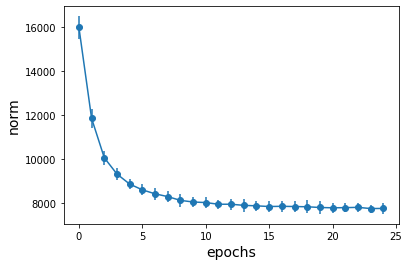
\includegraphics[scale=0.25]{figs/path-gram.png}
\caption{\label{fig:gen}$\nu_t=y^\top (\widehat{H}_t)^{-1} y$.}
\end{wrapfigure}
For a subset size, $n'=200$ ($100$ examples per class) we plot $\nu_t=y^\top (\widehat{H}_t)^{-1} y$, (where $y\in\{-1,1\}^{200}$ is the labeling function), and observe that $\nu_t$ reduces as training proceeds (see \Cref{fig:gen}). Note that, $\nu_t=\sum_{i=1}^{n'}(u_{i,t}^\top y)^2 (\hat{\rho}_{i,t})^{-1}$, where $u_{i,t}\in \R^{n'}$ are the orthonormal eigenvectors of $\widehat{H}_t$ and $\hat{\rho}_{i,t},i\in[n']$ are the corresponding eigenvalues. Since $\sum_{i=1}^{n'}\hat{\rho}_{i,t}=1$, the only way $\nu_t$ reduces is when more and more energy gets concentrated on $\hat{\rho}_{i,t}$s for which $(u_{i,t}^\top y)^2$s are also high.\WFclear%However, in $H_t=(x^\top x)\odot \lambda_t$, only $\lambda_t$ changes with time. Thus, $\lambda_t(s,s')$ which is a measure of overlap of sub-networks active for input examples $s,s'\in[n]$, changes in a manner to reduce $\nu_t$. We can thus infer that the \emph{right} active sub-networks are learned over the course of training.\\s
\begin{comment}\textbf{ReLU artefact:}In the case of ReLU activations (i.e., hard gates obtained for $\beta=\infty$ in \Cref{tb:dgn}), the gating values belong to $\{0,1\}$, and it follows that the activity $A_t(\cdot,\cdot)\in\{0,1\}$ and hence $\partial_{\tg} A_t(\cdot,\cdot)=0$. Consequently, there is no flow of the feature gradient in the GD update. However, since the gating parameter $\Tg$ identical with $\Theta$, (i.e., $\Tg_t=\Theta_t,\forall t$), $A_t$ changes with time due to the flow of the value gradient and NPF also changes with time. As a result, understanding feature learning in DNNs with ReLU activations is difficult, and we leave it for future work. In the next section, we study feature learning in parameterised DGNs with soft gates instead.
\end{comment}